\section{Data Analysis}

	% TODO@Christian: What is the bin-width and how did you determine it? Decide for one(!) time form: present OR simple past!
    According to the data evaluation, we got $N = 204$ events. That means, we got 204 times a distance, a time and a velocity which are distributed. 
    \subsection{Data evaluation of velocity}
        We think, the velocity is a gaussian distribution. This assumption can be proven by a student's t-test. But we only have one set of data.
        \begin{longtable}{p{8cm}p{8cm}}
            \minipanf
                A\\
                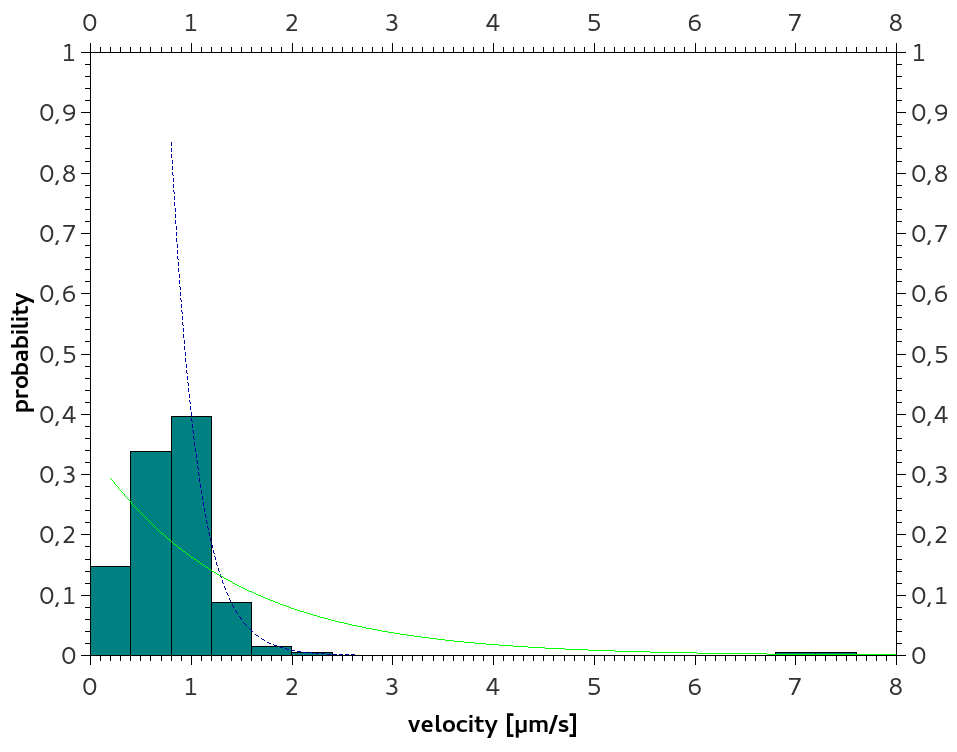
\includegraphics[scale=0.3]{pic/velodist_rel}
            \minipend
            &
            \minipanf
                B\\
                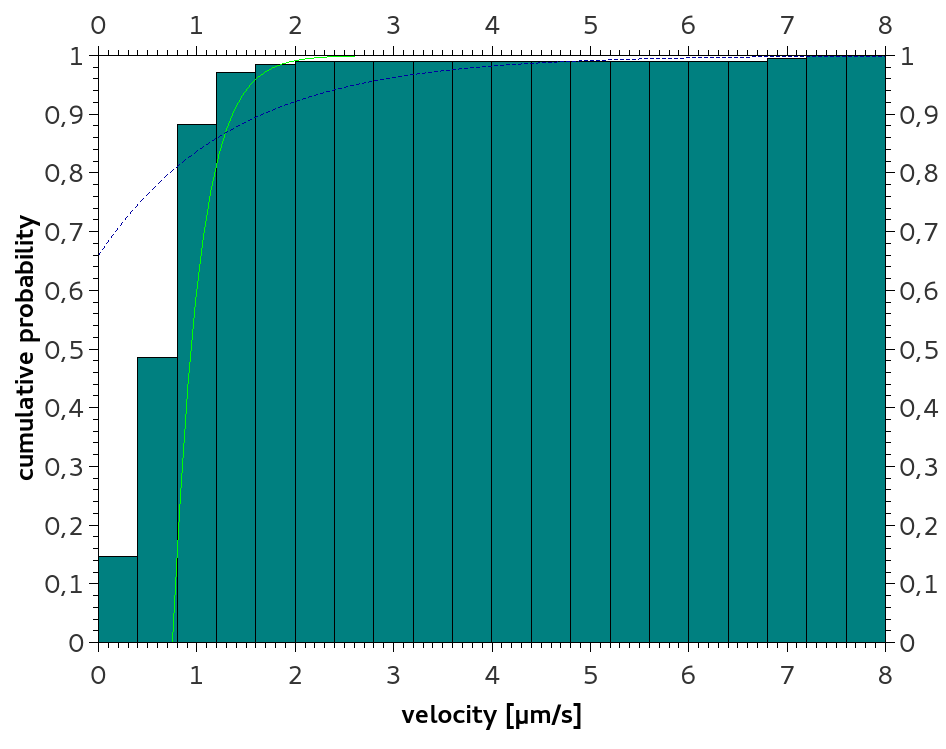
\includegraphics[scale=0.3]{pic/velocumdist}
            \minipend
        \end{longtable}
        \captionof{figure}{\textbf{A:} Histogram of the relative velocity distribution. \textbf{B:} Histogram of the cululative velocity distribution}
        \vspace{2mm}
        The mean of the velocity $\overline v$, its standard deviation $\sigma_{\overline v}$ and the standard error of the mean velocity $\Delta \overline v$ can be calculated by a data analysis tool. We used an Origin like software called qtiplot, which calculates column statistics, which are not influenced by binning, because that are the measured raw data. These include the searched values.
        In general one can calculate these values as following:
        \begin{eqnarray*}
            \overline v = N^{-1} \sum_{i = 1}^{N}v_i\ ,\ \sigma_{\overline v} = \sqrt{\sum_{i = 1}^{N} \frac{(v_i - \overline v)^2}{N-1}}\ , \ \Delta \overline v = \frac{\sigma_{\overline v}}{\sqrt{N}}
        \end{eqnarray*}
        So we get:
        $$ \overline v = \unit[(0.87 \pm 0.05)]{\frac{\mu m}{s}}\ , \ \ \sigma_{\overline v} = 0.72 \unit{\frac{\mu m}{s}}$$
        To minimize the error one could easily take more measurements. According to the law of large numbers the measured mean velocity would converge to the expactation value. With an infinite number of measurements we would get the exact result. 
        Also we could use software which marks the traces, which would create a unit law of marking. As a human being, one cannot see every trace and one can not mark every trace the way. This is caused by a diameter of the traces which is not infinite. The means, one could easily stretch the distance walked by the kinesin by marking from on edge to the diagonal opposite edge. An automization would avoid these errors. 
    
    \subsection{Data evaluation of run length}
    	Now we are going to figure out what distance $D$ a motorprotein covers on a single microtubule before releasing itself. For that we also use the data acquired by the streamed films. One frame of the stream corresponds to $150\ \unit{ms}$. With that and the determined velocity $\overline v = \unit[(0.87 \pm 0.05)]{\mu m/s}$ we can calculate the minimal distance we can measure with our streaming-system (and also the minimal bin-size): $d_{min} = \overline{v} \cdot 1\ \unit{FRAME} = 0.12\ \unit{\mu m} \cong 0.2\ \unit{\mu m}$. Therefore all of the measured distances which are below that value cannot be reasonable and they will be ignored in our statistics - anyway they will appear as first bin in the histogram for the sake of completeness. We rounded the value of $d_{min}$ up because we want to choose a smooth bin-width. Finally we decided the bin width to be $w_{bin} = 0.4\ \unit{\mu m} \cong 2 \cdot {d_{min}}$. We estimated this using the \textbf{Square-root choice}\cite{wikiHisto} which says that the number of bins is $k = \lfloor\sqrt{N}\rfloor$ where $N = 204$ is the number of samples.\\
    	Considering these facts we got the following results. At first the mean distance and its statistical error:
    	\begin{equation*}
    		\overline{D} = (1.1 \pm 0.1)\ \unit{\mu m}
    	\end{equation*}
    	The figures (\ref{exp:histRunLength}) and  (\ref{exp:cumuRunLength}) visualise the distribution of the measured distances:
    	 \minipanf
    	 	\centering
    	 	\captionsetup{justification=centering,margin=2cm}
    	 		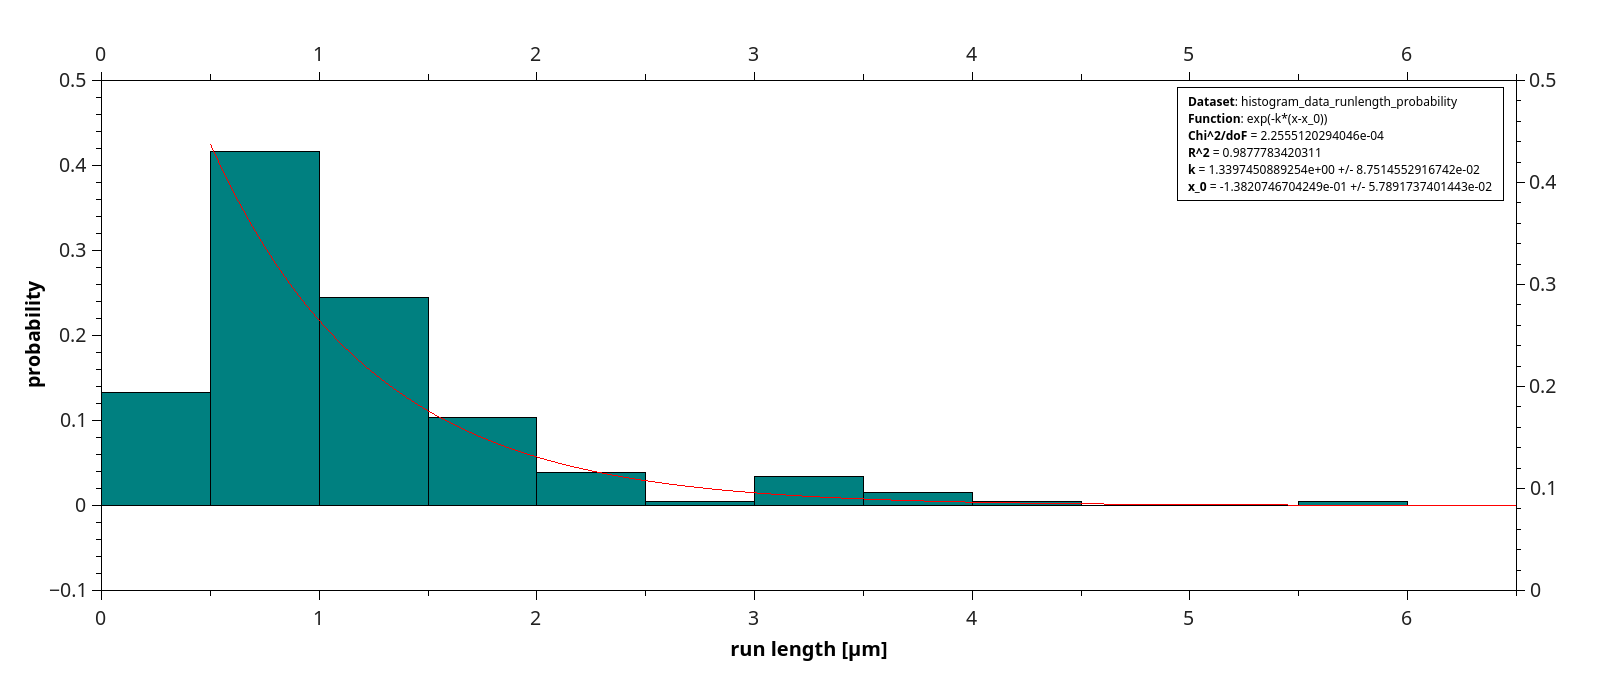
\includegraphics[width = 0.8\textwidth, keepaspectratio]{pic/histo_runlength_rel.png}
    	 	\caption{Probibility distribution of the measured run length.\\ The very first bin is ignored from the exponential fitting}
    	 	\label{exp:histRunLength}
    	 \minipend\\
    	 \ \\   
    	 Because all invalid values fall into the first bin, it will be disregarded in the exponential fit of the probability function $P_D(d)$ and in the cumulative probability. We consider this fact by using an offset $d_0 = w_{bin} = 2 \cdot d_{min} = 0.4\ \unit{\mu m}$ in the exponential fit of the probability distribution. So the fit equation becomes:
    	 \begin{equation*}
    	 	P_D(d) = A \cdot e^{-\kappa\cdot(d-d_0)}
    	 \end{equation*}
    	 with the fit parameters:
    	 \begin{align*}
    	  	&A = 0.37 \pm 0.02\\
    	  	&\kappa = (1.2 \pm 0.1)\ \unit{\mu m^{-1}}\\
    	  	&d_0 = 0.4\ \unit{\mu m}= \mathrm{const.}
    	 \end{align*}
    	 
    	 \minipanf
    	     	     \centering
    	     	     \captionsetup{justification=centering}            
    	     	         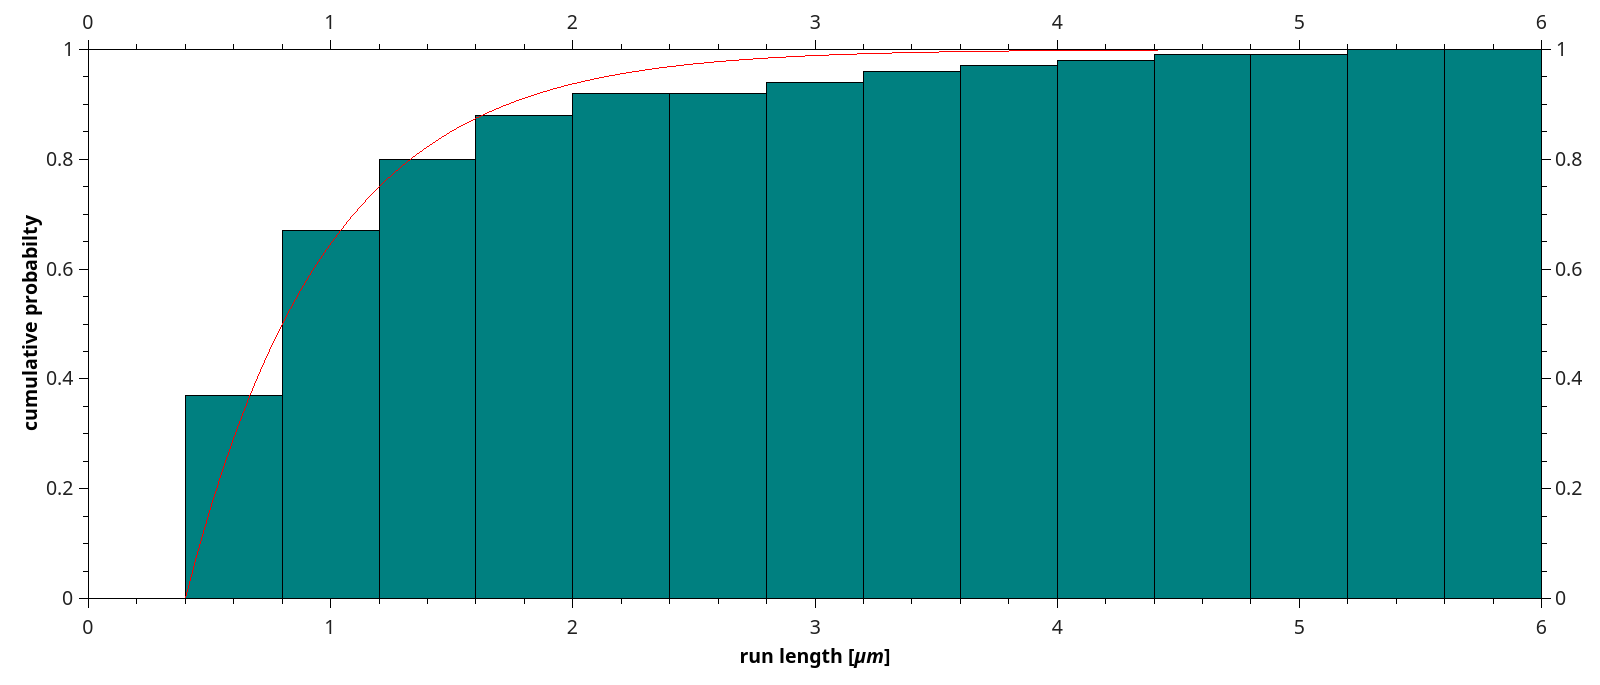
\includegraphics[scale=0.3]{pic/cumulative_runlength.png}
    	     	     \caption{Cumulative probability disregarding the 'invalid' values with $d < d_0$}
    	    			 \label{exp:cumuRunLength}             
    	 \minipend\\
    	 \ \\
    	 For the cumulative distribution function $F_D(d) = P_D(D \leq d)$ we use the fit equation:\\
    	 \begin{equation*}
    	     	 	F_D(d) = 1- e^{-k\cdot(d-d_0)}
    	 \end{equation*}
    	 and extract the fit parameters:
    	 \begin{align*}
    	     	  	&k = (1.7 \pm 0.4)\ \unit{\mu m^{-1}}\\
    	     	  	&d_0 = 0.4\ \unit{\mu m}= \mathrm{const.}
    	 \end{align*}
    	With that equation we can choose an arbitary confidence level $F_D(d)\overset{!}{=}\pi(d) \in [0,1]$ which gives the probability of the run length $D$ to be less or equal than given $d$. If we invert this function we get the \textit{characteristic run length} $d = \pi^{-1}(\pi(d))$:
    	\begin{align*}
    			&d(\pi) = d_0 + \ln((1-\pi)^{-1/k})\\
    			&\Delta d(\pi) = \abs{\frac{\partial d}{\partial k}\Delta k} = \abs{\frac{\Delta k}{k}\cdot(d_0 - d)} 
    	\end{align*}
    	We calculate this length for some characteristic values of $\pi$ that correspond to the confidence levels of the Gaussian normal distribution for finding the value of the random variable $x$ in an intervall around the expencted value:  $x \in [-n\sigma + \mu, n\sigma + \mu],\ n=1,2,3$:\\
    	\ \\
    	\minipanf
    		\centering
    		\begin{tabular}{c|c|c|c}
    	 	       $n$ & $\pi$ & $d(\pi)\ [\unit{\mu m}]$  & $\Delta d(\pi)\ [\unit{\mu m}]$\\
    	 	 \hline		1	& 	0.6827	&	1.1 	& 	0.2\\
    	  				2	&	0.9545	&	2.2		&	0.4\\
    	  				3	&	0.9973	&	3.9		& 	0.8	
    		\end{tabular}
    	\minipend\\
    	\ \\
    	We prefered the cdf-method to the pdf-method because we can check our result for given $\pi$ just by looking at the histogram without an additional integration. The deviation of the pdf-fit with respect to the histogram is also larger than in the cdf. We could minimise the error $\Delta d$ easily by taking more samples. We also should have avoided motorprotein-trajectories that are too 'short' to minimise the amount of values within the first bin. Also the magnification of the camera could be choosed larger to follow the trajectories better in the software